% =====================================================================
%  Лабораторная работа №3. Сплайн-интерполяция.
%  Вариант 4, таблица 4; X = 0.1838.
%
%  Сборка (любой из вариантов):
%      pdflatex  BastrakovReport.tex
%      xelatex   BastrakovReport.tex
%      lualatex  BastrakovReport.tex
%  (запускать два раза — для оглавления и перекрёстных ссылок)
% =====================================================================
\documentclass[14pt,a4paper]{extarticle}

% - Поддержка кириллицы: pdfLaTeX (T2A) либо XeLaTeX/LuaLaTeX (fontspec) -
\usepackage{iftex}
\ifPDFTeX
    \usepackage[T2A]{fontenc}
    \usepackage[utf8]{inputenc}
    \usepackage[russian]{babel}
    \usepackage{tempora}
    \usepackage{listingsutf8}
\else
    \usepackage{fontspec}
    \usepackage{polyglossia}
    \setdefaultlanguage{russian}
    \setotherlanguage{english}
    \IfFontExistsTF{Liberation Serif}%
        {\setmainfont{Liberation Serif}}%
        {\IfFontExistsTF{PT Serif}%
            {\setmainfont{PT Serif}}%
            {\setmainfont{TeX Gyre Termes}}}
    \IfFontExistsTF{DejaVu Sans Mono}%
        {\setmonofont{DejaVu Sans Mono}}%
        {\IfFontExistsTF{Liberation Mono}%
            {\setmonofont{Liberation Mono}}%
            {\setmonofont{TeX Gyre Cursor}}}
\fi

% - Математика, графика, оформление -----------
\usepackage{amsmath,amssymb}
\usepackage{graphicx}
\usepackage{geometry}
\usepackage{booktabs}
\usepackage{array}
\usepackage{float}
\usepackage{caption}
\usepackage{indentfirst}
\usepackage{xcolor}
\usepackage{listings}
\usepackage[hidelinks]{hyperref}

\geometry{a4paper,left=3cm,right=1.5cm,top=2cm,bottom=2cm}
\graphicspath{{graphics/img/}}

\captionsetup{labelsep=endash,justification=centering}
\setlength{\parindent}{1.25cm}
% Запас на растяжение строк: в XeLaTeX могут отсутствовать русские
% шаблоны переносов, поэтому длинные слова иначе вылезают за поля.
\setlength{\emergencystretch}{3em}
\tolerance=2000
\renewcommand{\arraystretch}{1.15}
\renewcommand{\labelenumi}{\arabic{enumi})}

% - Настройка листингов ---------------
\definecolor{lstgray}{gray}{0.45}
\definecolor{lstgreen}{rgb}{0.0,0.45,0.0}
\definecolor{lstblue}{rgb}{0.05,0.15,0.55}
\definecolor{lstred}{rgb}{0.6,0.1,0.1}

\lstset{
    basicstyle=\ttfamily\footnotesize,
    language={[Sharp]C},
    breaklines=true,
    frame=single,
    numbers=left,
    numberstyle=\tiny\color{lstgray},
    keywordstyle=\color{lstblue}\bfseries,
    commentstyle=\color{lstgreen}\itshape,
    stringstyle=\color{lstred},
    showstringspaces=false,
    tabsize=4,
    captionpos=b,
    columns=fullflexible,
    keepspaces=true,
}

\newcommand{\includecode}[1]{%
    \ifPDFTeX
        \ifcsname lst@UseInputEncoding\endcsname
            \lstinputlisting[inputencoding=utf8]{#1}%
        \else
            \lstinputlisting{#1}%
        \fi
    \else
        \lstinputlisting{#1}%
    \fi
}

\begin{document}

% =====================================================================
%  Титульный лист
% =====================================================================
\begin{titlepage}
    \centering
    \large
    Министерство образования и науки РФ\\[0.3cm]
    Пермский национальный исследовательский политехнический университет\\[0.3cm]
    Электротехнический факультет\\[0.3cm]
    Кафедра "Информационные технологии и автоматизированные системы"

    \vspace{3.5cm}
    {\Large Информатика в приложении к отрасли}\\[0.4cm]
    {\Large\bfseries Лабораторная работа № 3}\\[0.6cm]

    Тема: "Сплайн-интерполяция"\\[0.2cm]
    Вариант 4

    \vspace{4.5cm}
    \begin{flushleft}
        \large
        Выполнил: студент группы РИС-25-2б \hfill Бастраков Данил\\[0.5cm]
        Проверил: профессор кафедры ИТАС \hfill Шварц К.~Г.\\[0.5cm]
        Дата: \underline{\hspace{3cm}} \hfill Подпись: \underline{\hspace{4cm}}
    \end{flushleft}

    \vfill
    Пермь\\ 2026
\end{titlepage}

\tableofcontents
\newpage

% =====================================================================
\section{Постановка задачи}
% =====================================================================

\textbf{Цель работы} --- вычислить приближённое значение функции,
заданной таблично, в точке $X$ с помощью кубического сплайна и
реализовать соответствующий алгоритм в программе.

Дана таблица значений функции $y(x)$ (вариант~4, таблица~4):
\begin{equation}
\begin{array}{c|cccccc}
    x_i & 0{,}180 & 0{,}185 & 0{,}190 & 0{,}195 & 0{,}200 & 0{,}205\\
    \hline
    y_i & 5{,}61543 & 5{,}46693 & 5{,}32634 & 5{,}19304 & 5{,}06649 & 4{,}94619
\end{array}
\label{eq:data}
\end{equation}

Требуется найти приближённое значение $y(0{,}1838)$.

Перед решением необходимо убедиться, что узлы образуют возрастающую
сетку:
\[
    0{,}180 < 0{,}185 < 0{,}190 < 0{,}195 < 0{,}200 < 0{,}205 .
\]
Точка $X=0{,}1838$ принадлежит первому отрезку
$[0{,}180;\,0{,}185]$, поэтому для вычисления используется первый
кубический многочлен сплайна.

% =====================================================================
\section{Краткое описание метода}
% =====================================================================

\subsection{Кубический сплайн}

Кубическим сплайном дефекта~1 с узлами $x_1,\ldots,x_n$ называется
функция $S(x)$, которая на каждом отрезке $[x_i,x_{i+1}]$ является
многочленом третьей степени
\begin{equation}
    S_i(x)=a_i+b_i(x-x_i)+c_i(x-x_i)^2+d_i(x-x_i)^3,
    \qquad x\in[x_i,x_{i+1}],
    \label{eq:spline}
\end{equation}
непрерывна вместе с первой и второй производными во всех внутренних
узлах и удовлетворяет условиям интерполяции
\begin{equation}
    S_i(x_i)=y_i,\qquad S_i(x_{i+1})=y_{i+1}.
    \label{eq:interp}
\end{equation}

Для однозначного определения сплайна зададим естественные граничные
условия нулевой кривизны на концах:
\begin{equation}
    S''(x_1)=0,\qquad S''(x_n)=0.
    \label{eq:natural}
\end{equation}

\subsection{Определение вторых производных в узлах}

Обозначим $m_i=S''(x_i)$ и $h_i=x_{i+1}-x_i$. Из условий
\eqref{eq:interp} и требований непрерывности первой производной во
внутренних узлах получается трёхдиагональная система для $m_i$:
\begin{equation}
    \begin{cases}
        m_1=0,\\[2mm]
        h_{i-1}m_{i-1}+2(h_{i-1}+h_i)m_i+h_i m_{i+1}
        =6\left(\dfrac{y_{i+1}-y_i}{h_i}
        -\dfrac{y_i-y_{i-1}}{h_{i-1}}\right),\\[3mm]
        m_n=0,
    \end{cases}
    \label{eq:system}
\end{equation}
(второе уравнение записано для $i=2,\ldots,n-1$).

После нахождения $m_i$ коэффициенты сплайна \eqref{eq:spline}
вычисляются по формулам
\begin{equation}
    a_i=y_i,\qquad
    c_i=\frac{m_i}{2},\qquad
    d_i=\frac{m_{i+1}-m_i}{6h_i},
    \label{eq:coeff-cd}
\end{equation}
\begin{equation}
    b_i=\frac{y_{i+1}-y_i}{h_i}
    -\frac{h_i}{6}\left(2m_i+m_{i+1}\right).
    \label{eq:coeff-b}
\end{equation}

\subsection{Метод прогонки}

Система \eqref{eq:system} имеет трёхдиагональную матрицу
\begin{equation}
    a_i z_{i-1}+b_i z_i+c_i z_{i+1}=d_i,\qquad 1\le i\le n,
    \label{eq:tridiag}
\end{equation}
где $a_1=0$, $c_n=0$, а $z_i$ --- искомые $m_i$. Матрица системы
строго диагонально преобладает: для внутренних уравнений
$2(h_{i-1}+h_i)>h_{i-1}+h_i$, а крайние уравнения имеют единичную
диагональ. Поэтому метод прогонки устойчив и знаменатели
$a_ip_{i-1}+b_i$ не обращаются в нуль. Решение ищется в виде
\begin{equation}
    z_i=p_i z_{i+1}+q_i .
    \label{eq:sweep-form}
\end{equation}
Прямой ход метода прогонки:
\begin{equation}
    p_1=-\frac{c_1}{b_1},\qquad q_1=\frac{d_1}{b_1},
    \label{eq:sweep-start}
\end{equation}
\begin{equation}
    p_i=-\frac{c_i}{a_i p_{i-1}+b_i},\qquad
    q_i=\frac{d_i-a_i q_{i-1}}{a_i p_{i-1}+b_i},
    \qquad i=2,\ldots,n-1.
    \label{eq:sweep-forward}
\end{equation}
Обратный ход:
\begin{equation}
    z_n=q_n,\qquad z_i=p_i z_{i+1}+q_i,\quad i=n-1,\ldots,1.
    \label{eq:sweep-back}
\end{equation}

% =====================================================================
\section{Исходные данные для расчёта}
% =====================================================================

Данные варианта~4 (таблица~4) и шаги сетки приведены в
табл.~\ref{tab:data}. Все шаги одинаковы: $h_i=0{,}005$.

\begin{table}[H]
    \centering
    \caption{Исходная таблица и шаги сетки}
    \label{tab:data}
    \begin{tabular}{crrr}
        \toprule
        $i$ & $x_i$ & $y_i$ & $h_i$\\
        \midrule
        1 & 0{,}180 & 5{,}61543 & 0{,}005\\
        2 & 0{,}185 & 5{,}46693 & 0{,}005\\
        3 & 0{,}190 & 5{,}32634 & 0{,}005\\
        4 & 0{,}195 & 5{,}19304 & 0{,}005\\
        5 & 0{,}200 & 5{,}06649 & 0{,}005\\
        6 & 0{,}205 & 4{,}94619 & ---\\
        \bottomrule
    \end{tabular}
\end{table}

% =====================================================================
\section{Результаты вычислений}
% =====================================================================

\subsection{Система для вторых производных}

При $n=6$ система \eqref{eq:system} содержит шесть неизвестных
$m_1,\ldots,m_6$. Её коэффициенты и правые части приведены в
табл.~\ref{tab:system}.

\begin{table}[H]
    \centering
    \caption{Трёхдиагональная система для $m_i$}
    \label{tab:system}
    \small
    \begin{tabular}{crrrr}
        \toprule
        $i$ & $a_i$ & $b_i$ & $c_i$ & $d_i$\\
        \midrule
        1 & 0        & 1     & 0     & 0\\
        2 & 0{,}005  & 0{,}020 & 0{,}005 & 9{,}492\\
        3 & 0{,}005  & 0{,}020 & 0{,}005 & 8{,}748\\
        4 & 0{,}005  & 0{,}020 & 0{,}005 & 8{,}100\\
        5 & 0{,}005  & 0{,}020 & 0{,}005 & 7{,}500\\
        6 & 0        & 1     & 0     & 0\\
        \bottomrule
    \end{tabular}
\end{table}

\subsection{Прямой и обратный ход прогонки}

По формулам \eqref{eq:sweep-start}--\eqref{eq:sweep-back} получены
прогоночные коэффициенты, приведённые в табл.~\ref{tab:sweep}.
После обратного хода найдены вторые производные в узлах
(табл.~\ref{tab:m}).

\begin{table}[H]
    \centering
    \caption{Прогоночные коэффициенты}
    \label{tab:sweep}
    \small
    \begin{tabular}{crr}
        \toprule
        $i$ & $p_i$ & $q_i$\\
        \midrule
        1 & $-0{,}000000$ & $0{,}000000$\\
        2 & $-0{,}250000$ & $474{,}600000$\\
        3 & $-0{,}266667$ & $339{,}999999$\\
        4 & $-0{,}267857$ & $342{,}857143$\\
        5 & $-0{,}267943$ & $310{,}047847$\\
        6 & $-0{,}000000$ & $0{,}000000$\\
        \bottomrule
    \end{tabular}
\end{table}

\begin{table}[H]
    \centering
    \caption{Вторые производные в узлах}
    \label{tab:m}
    \begin{tabular}{crr}
        \toprule
        $i$ & $x_i$ & $m_i$\\
        \midrule
        1 & 0{,}180 & 0\\
        2 & 0{,}185 & 406{,}920574\\
        3 & 0{,}190 & 270{,}717703\\
        4 & 0{,}195 & 259{,}808612\\
        5 & 0{,}200 & 310{,}047847\\
        6 & 0{,}205 & 0\\
        \bottomrule
    \end{tabular}
\end{table}

\subsection{Коэффициенты сплайна}

По формулам \eqref{eq:coeff-cd}--\eqref{eq:coeff-b} вычислены
коэффициенты многочленов на всех отрезках (табл.~\ref{tab:coeff}).

\begin{table}[H]
    \centering
    \caption{Коэффициенты кубического сплайна}
    \label{tab:coeff}
    \footnotesize
    \begin{tabular}{clrrrr}
        \toprule
        $i$ & отрезок & $a_i$ & $b_i$ & $c_i$ & $d_i$\\
        \midrule
        1 & $[0{,}180;0{,}185]$ & 5{,}615430 & $-30{,}039100$ & 0{,}000000 & 13564{,}019139\\
        2 & $[0{,}185;0{,}190]$ & 5{,}466930 & $-29{,}021799$ & 203{,}460287 & $-4540{,}095694$\\
        3 & $[0{,}190;0{,}195]$ & 5{,}326340 & $-27{,}327703$ & 135{,}358852 & $-363{,}636364$\\
        4 & $[0{,}195;0{,}200]$ & 5{,}193040 & $-26{,}001388$ & 129{,}904306 & 1674{,}641148\\
        5 & $[0{,}200;0{,}205]$ & 5{,}066490 & $-24{,}576746$ & 155{,}023923 & $-10334{,}928230$\\
        \bottomrule
    \end{tabular}
\end{table}

\subsection{Значение в точке $X$}

Точка $X=0{,}1838$ лежит на первом отрезке
$[0{,}180;\,0{,}185]$. Поэтому
\[
    dx=X-x_1=0{,}1838-0{,}180=0{,}0038.
\]
Подставляя коэффициенты первой строки табл.~\ref{tab:coeff} в
формулу \eqref{eq:spline}, получаем
\begin{align*}
    S(0{,}1838)
    &=5{,}615430-30{,}039100\cdot0{,}0038\\
    &\quad+0\cdot0{,}0038^2
      +13564{,}019139\cdot0{,}0038^3\\
    &=5{,}502025703.
\end{align*}

Таким образом,
\[
    \boxed{y(0{,}1838)\approx S(0{,}1838)=5{,}502025703.}
\]

\subsection{Проверка в узлах}

В табл.~\ref{tab:check} приведены значения сплайна в узловых точках.
Они совпадают с табличными значениями, что подтверждает выполнение
условий интерполяции \eqref{eq:interp}.

\begin{table}[H]
    \centering
    \caption{Проверка значений сплайна в узлах}
    \label{tab:check}
    \begin{tabular}{crrrr}
        \toprule
        $i$ & $x_i$ & $y_i$ & $S(x_i)$ & $|S(x_i)-y_i|$\\
        \midrule
        1 & 0{,}180 & 5{,}61543 & 5{,}615430 & 0\\
        2 & 0{,}185 & 5{,}46693 & 5{,}466930 & 0\\
        3 & 0{,}190 & 5{,}32634 & 5{,}326340 & 0\\
        4 & 0{,}195 & 5{,}19304 & 5{,}193040 & 0\\
        5 & 0{,}200 & 5{,}06649 & 5{,}066490 & 0\\
        6 & 0{,}205 & 4{,}94619 & 4{,}946190 & 0\\
        \bottomrule
    \end{tabular}
\end{table}

График табличных точек и построенного сплайна приведён на
рис.~\ref{fig:spline}.

\begin{figure}[H]
    \centering
    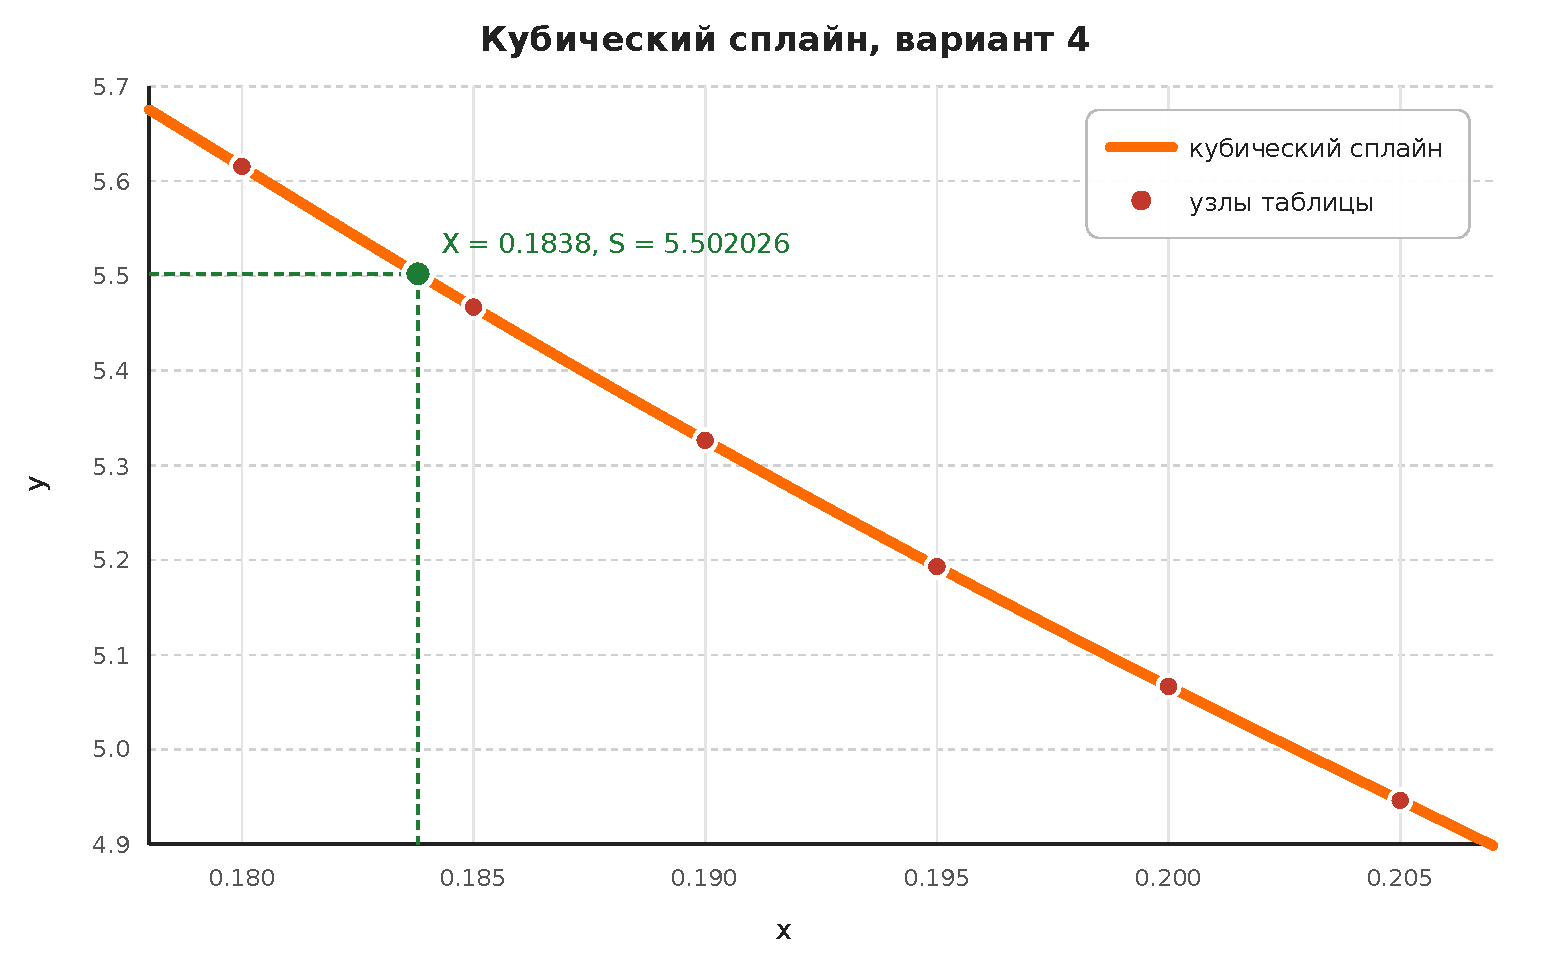
\includegraphics[width=0.9\textwidth]{fig_spline.pdf}
    \caption{Кубический сплайн для таблицы варианта~4 и точка $X=0{,}1838$}
    \label{fig:spline}
\end{figure}

% =====================================================================
\section{Обсуждение результатов}
% =====================================================================

Полученное значение $S(0{,}1838)=5{,}502025703$ лежит между
табличными значениями $y_1=5{,}61543$ и $y_2=5{,}46693$, что
согласуется с поведением функции на рассматриваемом отрезке.

Для сравнения, линейная интерполяция по первым двум узлам даёт
\[
    y_{\text{лин}}(0{,}1838)
    =5{,}61543+\frac{5{,}46693-5{,}61543}{0{,}005}\cdot0{,}0038
    =5{,}502570.
\]
Разность со сплайном составляет примерно $0{,}000544$, то есть
кубический сплайн учитывает кривизну функции и даёт более гладкое
приближение, чем линейная интерполяция.

Внутренние вторые производные $m_i$ положительны, поэтому на
рассматриваемом участке сплайн выпукл вниз. Производная сплайна в
точке $X$ равна приближённо
\[
    S'(0{,}1838)\approx-29{,}452,
\]
то есть функция убывает, что соответствует исходной таблице.

Для оценки точности сравним полученный результат со сплайном,
построенным только по первым пяти узлам ($0{,}180$--$0{,}200$):
\[
    S_5(0{,}1838)=5{,}502018297, \qquad
    |S(0{,}1838)-S_5(0{,}1838)|\approx 7{,}4\cdot10^{-6}.
\]
Столь малое изменение при добавлении шестого узла согласуется с
порядком аппроксимации кубического сплайна $O(h^4)$: при
$h=0{,}005$ величина $h^4\approx6{,}25\cdot10^{-10}$, а оценка по
четвёртой разделённой разности даёт погрешность порядка
$10^{-6}$.

Все узловые значения воспроизводятся точно (в пределах машинной
погрешности), система для вторых производных решена с невязкой, не
превосходящей $10^{-12}$. Это подтверждает корректность построения
сплайна и реализации метода прогонки.

\end{document}
